\begin{figure}[t!]
\vspace{-10px}
\centering
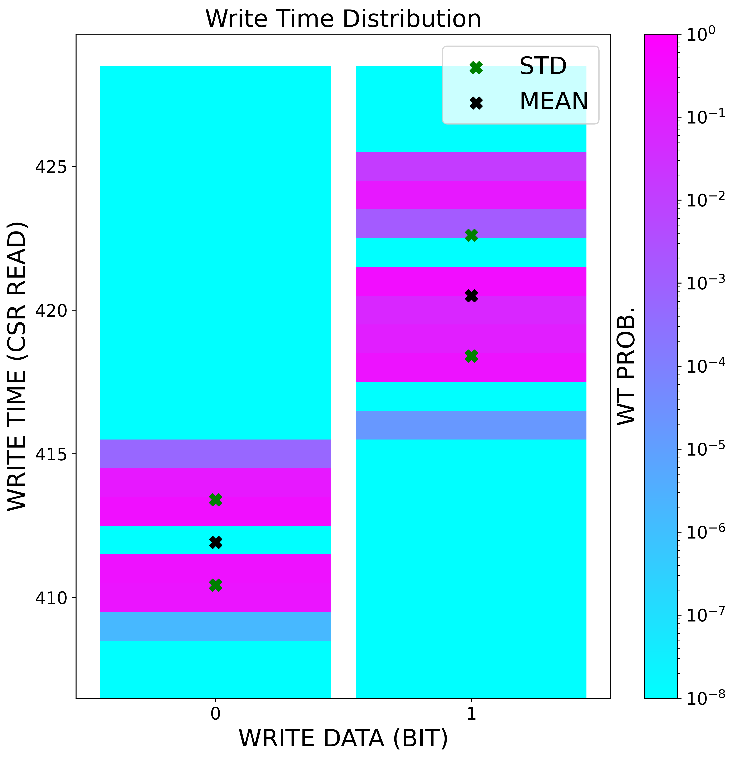
\includegraphics[width=0.75\linewidth]{img/full_chip_single_bit_dist.png}
\caption{Distribution of logical 0/1 DUT single bit write times. The memory is initialized completely to logical 0. Every bit in the memory array is toggled 20 times and the write time distribution is recorded. The distribution is expressed as a heat bar where strips are sized according to the measurement resolution (the time to poll the CSR). The color of each strip represents the probability of observing a write completion after a number of CSR reads\label{fig:ful_chip_single_bit}}
\end{figure} 